\documentclass[]{nsm-thesis}
% options:
% [germanthesis] - Thesis is written in German
% [plainunnumbered] - Don't print numbers on plain pages
% [earlydraft] - Settings for quick draft printouts
% [watermark] - Print current time/date at bottom of each page
% [phdthesis] - switch to PhD thesis style
% [twoside] - double sided
% [cutmargins] - text body fills complete page

% Author name. Separate multiple authors with commas.
\author{Dmitriy Monakhov}
\birthday{28. April 1999}
\birthplace{Moscow}

% Title of your thesis.
\title{Improving Urban Traffic Flow with Drone Supported Vehicular Networks}

\thesistype{Master's Thesis in Distributed Systems Engineering}\thesiscite{Master's Thesis~(Masterarbeit)}

\advisors{Mario Franke, Christoph Sommer}
% List of advisors (without academic titles), separated by commas.

% List of referees (without academic titles), separated by commas.
\referees{Christoph Sommer, Burkhard Hensel}


% Define abbreviations used in the thesis here.
\acrodef{DAVN}{Drone-assisted vehicular network}
\acrodef{LOS}{Line of sight}
\acrodef{MANET}{Mobile Ad Hoc Network}
\acrodef{VANET}{Vehicular Ad Hoc Network}
\acrodef{OSG}{OpenSceneGraph}
\acrodef{MAC}{Medium access control}
\acrodef{NIC}{Network interface controller}
\acrodef{DSRC}{Dedicated Short-Range Communications}
\acrodef{V2V}{Vehicle-to-vehicle}
\acrodef{V2I}{Vehicle-to-infrastructure}
\acrodef{V2D}{Vehicle-to-drone}
\acrodef{D2D}{Drone-to-drone}
\acrodef{GUI}{Graphical User Interface}
\acrodef{TraCI}{Traffic Control Interface}
\acrodef{ATR}{Average Transmission Range}
\acrodef{NS-2}{Network Simulator 2}
\acrodef{FCC}{Federal Communications Commission}
%\acrodef{ROI}{Region of Interest}{short-indefinite={an}, long-plural-form={Regions of Interest}}
%\acrodef{ADAC}{German Automobile Association}{foreign={Allgemeiner Deutscher Automobilclub}}
%\acrodef{CANhashing}[CAN]{Content Addressable Network}{extra={when referring to the distributed hash table}}
%\acrodef{CANproto}[CAN]{Controller Area Network}{extra={when referring to the bus protocol}}

\begin{document}

\pagenumbering{roman}

\maketitle

\cleardoublepage


\chapter*{Abstract}
\addcontentsline{toc}{chapter}{Abstract}
\begin{otherlanguage*}{american}

In future cities will probably be populated with smart autonomous vehicles, communicating with each other and forming so called vehicular ad hoc networks. Among other uses, these networks can be used to broadcast safety or traffic-control messages in order to improve situational awareness of vehicles, which can be used to improve the traffic flow. The problem is, that in high-density urban development the buildings highly obstruct vehicle-to-vehicle communications. One possible solution is usage of drone-assisted vehicular networks. The drones can help via rebroadcasting messages across the city blocks to another streets, where other drones or vehicles will receive them. The main advantage of drones is the ease with which they can maintain line-of-sight with vehicles and each other.

In this work I explored a scenario, where drones fly opportunistically above the city and rebroadcast messages, that are sent by broken down vehicles. This way multi-hop transmission lines are established between vehicles on the scene. Receiving vehicles will adjust their routes in order to avoid traffic jams. The software simulation was built to find out the effects of drones in this case, how can they improve the traffic flow. Several metrics like average vehicle speed, number of jammed vehicles and time in jam were evaluated.

The simulation results showed significant improvement in traffic flow in all considered metrics. The drones are able to maintain line-of-sight with vehicles even without special navigation algorithms applied. Therefore, with drones the messages are better transmitted in urban environment, which, in conclusion, means that opportunistically flying drones can be used in urban environments in order to improve the vehicular traffic flow in the covered area.

\end{otherlanguage*}

\acresetall

\cleardoublepage
\setcounter{tocdepth}{1}
\tableofcontents

\cleardoublepage
\pagenumbering{arabic}



\chapter{Introduction}
%\chapter{Einleitung}
\label{sec:introduction}

Current technology already enables us to create semi-autonomous vehicles. Although, for now fully-autonomous vehicles are rarely allowed to 
populate the roads, in future it will probably be possible. One perspective option for autonomous driving are cooperative autonomous vehicles: such machines
that can drive on their own and maintain situation-awareness via communicating with other vehicles on the roads.

Since our world is rapidly urbanizing, it will be desirable to enable autonomous vehicles to drive in large cities. And there is a problem here: communication between vehicles will be difficult in urban areas. In cities, buildings stand close to each other. Buildings are usually built of radio-opaque materials. At the same time, the buildings are quite massive. Thus, it turns out that the propagation of radio signals between low-power vehicle transmitters becomes very difficult if the cars are not on the same street. This leads to communication outages in \ac{V2V} networks operating inside urban areas.

One possible solution to this problem could be drones. Cities of the future will probably be populated by autonomous drones flying in the air above the roofs of buildings. This gives drones the advantage of making it much easier for them to maintain a line of sight between each other and with vehicles on the ground. Consequently, their radio transmissions are less likely to be blocked by buildings. In this way, drones can help vehicles spread signals better, bypassing buildings standing between the vehicles.

In this paper, I explore whether there is an advantage in connecting a network of opportunistically flying drones to a network of vehicles in terms of assisting with urban vehicular traffic via rebroadcasting jamming announcements from broken vehicles.
Since a real-life experiment will be too expensive and difficult to conduct, I will use software simulation.

\chapter{Fundamentals}
\label{sec:fundamentals}

In this section, I will explain the basic terms, technologies and methods that will be used later. But first, I am going to review available literature to show current state-of-the-art in drone-assisted vehicular vehicles and show what is new in my project.


\section {Related Work}

\acp{DAVN} are already known in literature, however the proposed purpose and role of drones differ from work to work. \textcite{shi2018drone} propose an architecture for a \ac{DAVN} and provide experimental proof that drones can improve networking between the vehicles. In particular, the authors show improved communication throughput and delay. The authors discuss different drone roles, use cases for \acp{DAVN} and three types of \ac{DAVN}: Drone Swarm Network, Drone Assisted \ac{V2I} and Drone Assisted \ac{V2V}. The \ac{V2I} type describes how drones can assist in expanding the coverage of preexisting infrastructure. The proposed drone-swarming architecture describes \ac{D2D} links used by drones to avoid collisions and calculate safe flying paths. The last one, Drone Assisted \ac{V2V}, is closely related to my project. The authors explain, that in Drone Assisted \ac{V2V} the drones try to maintain the \ac{LOS} with the vehicles in order to assist with message broadcasting. The drones relay messages from vehicles to other drones and vehicles. The architecture is somewhat similar to mine, however, my work differs in the simulation setup, used software and goals. At first, \textcite{shi2018drone} use a static pre-generated traffic flow using PTV VISSIM. In my work another traffic simulator (SUMO) is used, and the routes are dynamic. Since I am trying to evaluate, how the drones can assist in improving the traffic flow, my vehicles can regenerate and change the routes according to incoming information. Second, in the scenario of \textcite{shi2018drone} the authors use a long straight bidirectional highway. In contrast, I use a road grid with dense urban environment. Third, I use OMNeT++ as a network simulator, when they use \ac{NS-2}. \textcite{shi2018drone} use the simulation to evaluate the improvement of networking, but my main goal is to check, how drones help to avoid traffic jams in an environment, where \ac{V2V} communications are highly obstructed.

\textcite{peng2021edge} propose an architecture, where drones are used to assist in computations, needed for autonomous vehicles. The authors argue, that an AI-based resource management system can dynamically allocate drones to areas, where a demand for computational power is high. The authors also conduct a case-study to demonstrate the performance of applying AI technologies in resource management. Another work focusing on similar issue is \textcite{Wu2020Caching}. In this work the authors propose a technique allowing drones to be used as caches for heavy data. This technique tries to adjust the drones' locations in order to solve the problems of content placement and delivery.

Many works like \textcite{lin2020novel} focus on analyzing and improving the \ac{VANET} network connectivity using drones. In the cited article the authors propose an algorithm that dispatches the drones to the most appropriate locations in real-time according to the predicted distribution of the vehicles. To show the improvements, the authors conducted simulations, which test the network performance based on the real map data. Another example is \textcite{khabbaz2019modeling}, where the authors seek to analyze and model benefits for vehicular networking performance, derived from using off-road relays like drones or road-side units. In \textcite{tariq2020imoc} the problem of routing is discussed. The authors try to improve routing performance using an AI-based clustering algorithm in order to provide an optimal route with minimum overhead.

A couple of works focus on connecting the \acp{DAVN} to another networks. For example, \textcite{saputro2018security} propose a mechanism to integrate \ac{DAVN} into existing LTE infrastructure.

\textcite{Khabbaz2021Multihop} investigate a setup similar to mine: the drones opportunistically fly above the vehicles and serve as flying base stations responsible for routing vehicle data. The work discusses how the communications between vehicles can be done using multi-hop paths connecting vehicles and drones. However, the goal of their work is to improve the network connectivity, while my goal is to evaluate improvements in traffic flow.

There are several related articles by Oubbati, working in an environment, similar to mine.
In \cite{Oubbati2021Dispatch} the authors explore the improvements that drones can give to \ac{VANET} networking and propose an algorithm to dispatch drones to cover maximum area. The authors focus on urban environment, but, in contrast to my work, evaluate networking performance, coverage and energy consumption and do not consider traffic flow improvements. In \cite{Oubbati2016intersection} the authors propose a drone-placement algorithm that improves routing performance and network connectivity in urban intersections. Article \cite{OUBBATI201793} also describes similar issue, exploring routing protocols in urban \acp{VANET} and describing improvements for the protocol, proposed in \cite{Oubbati2016intersection}.

I have listed multiple current works above, and none on them explore the possibility of drones improving the traffic flow and only few of them use urban environments. Although, the field of \acp{DAVN} is rapidly developing, it seems like there is little research of this particular scenario. Therefore, I will explore this area and show experimental evidence that drones can help with improving the traffic in dense cities.


\section{Ad hoc networks}

In order to understand my work properly, the reader should know some basic terms. In this and following sections I will describe these terms briefly. The central technology, which is a basis of \acp{DAVN} is the ad hoc network. A good definition of ad hoc networks was given by Ram Ramanathan and Jason Redi in IEEE communications Magazine \cite{ramanathan2002brief}: An ad hoc network is a (possibly mobile) collection of communications devices (nodes) that wish to communicate, but have no fixed infrastructure available, and have no pre-determined organization of available links. The authors explain that individual nodes are responsible for dynamically discovering which other nodes they can directly communicate with, and the nodes are required to relay packets on behalf of other nodes in order to deliver data across the network.

According to Toor et al \cite{toor2008}, Vehicular ad hoc network (\ac{VANET}) is a special case of a mobile ad hoc network, where communication links are formed between the vehicles.



\section{Broadcast Storm}

A common challenge in implementing mobile ad hoc networks (including \acp{VANET}), according to \textcite{wisitrophan2007} is the broadcast storm. Authors define the broadcast storm as a frequent contention and collisions in transmission among neighboring nodes, when the nodes unconditionally broadcast packets. Authors further argue, that multiple solutions exist to alleviate this problem in usual \ac{MANET} environment, but only few are suitable to resolve the broadcast storm issue in \ac{VANET} context.

In my work the broadcast storm is also an issue that needs to be addressed. In my scenario the broadcast storm would be observed between vehicles and between drones if no suppression technique is present. At first, I will list some location-based techniques, explored by \textcite{wisitrophan2007} for vehicular ad hoc networks and choose the one that is suitable for my scenario.

\begin{itemize}

\item \emph{Weighted p-Persistence Broadcasting} - Each node rebroadcasts a packet with a probability that is directly proportional to the distance to the sending node. Duplicate packets are discarded. \cite[Page~88]{wisitrophan2007}.

\item \emph{Slotted 1-Persistence Broadcasting} - The delay before a packet is rebroadcast depends on the distance to the sending node. Unique packets are always rebroadcast, duplicate packets are discarded. \cite[Page~88]{wisitrophan2007}.

\item \emph{Slotted p-Persistence Broadcasting} - The delay before a packet is rebroadcast depends on the distance to the sending node. Unique packets are rebroadcast with a predetermined probability, duplicate packets are discarded. \cite[Page~89]{wisitrophan2007}.

\end{itemize}

\textcite{wisitrophan2007} also discuss Received-Signal-Strength-Based broadcast suppression schemes, but since in my work it is assumed that the vehicles always know their exact location and location-based algorithms can be used, these techniques are not relevant.

\subsection{Weighted p-Persistence Broadcasting}

In my work I will use the Weighted p-Persistence for both vehicles and drones, because it is the simplest to implement, and it shows sufficient performance in my scenario. In this section I will describe Weighted p-Persistence Broadcasting in more detail and explain the choice of some parameters.

According to \textcite{wisitrophan2007}, the rule of Weighted p-Persistence can be described like this: Upon receiving a packet from node \emph{i}, node \emph{j} checks the packet ID and rebroadcasts with probability $p_{ij}$ if it receives the packet for the first time; otherwise, it discards the packet.

The formula for calculating $p_{ij}$ looks like this:

\begin{equation}\label{eq:bs-p}
p_{ij} = \frac{D_{ij}}{R}
\end{equation}

where \emph{R} is the average transmission range and $D_{ij}$ is relative distance between nodes \emph{i} and \emph{j}. Authors further add, that if a node receives duplicate packets from multiple sources within the waiting period \emph{WAIT\textunderscore TIME} before rebroadcasting, this node selects the smallest $p_{ij}$ value as rebroadcasting probability. Authors clarify, that this means that nodes use the relative distance to the nearest broadcaster in order to ensure that nodes who are farther away rebroadcast with higher probability. Additionally, authors propose a method to prevent the messages from dying out: if a node decides not to rebroadcast, it keeps the message for time WAIT\textunderscore TIME + $\delta$, where $\delta$ is the one-hop transmission and propagation delay. If a node does not receive a packet from somebody else, it rebroadcasts it with probability 1 after WAIT\textunderscore TIME + $\delta$.

In my scenario, I will use different \emph{R} values for vehicles and drones. On one hand, since drones maintain the line-of-sight with each other, the R can be relatively large for them, slightly less than there maximum transmission range. On the other hand, vehicles can only communicate withing the length of the street they are standing on. Therefore, the \emph{R} for vehicles will be roughly equal to the length of a city block (distance between two crossroads in a grid, which is much smaller than maximum possible transmission range of a vehicle). This way vehicles, that are standing near two crossroads will rebroadcast with probability around 1. This will ensure that messages can "turn around" the buildings with higher probability.





\section {Simulation Software}

As it was mentioned earlier, conducting a full-scale real-life experiment will be very expensive. Therefore, a good idea is to use software to simulate the scenario and evaluate the results. 

There are multiple network simulators available on the market. A survey, conducted by \textcite{pan2008survey} contains a list of most popular tools:
\begin{itemize}
\item OPNET \cite[Page~5]{pan2008survey}
\item Network Simulator 2 \cite[Page~7]{pan2008survey}
\item Network Simulator 3 \cite[Page~8]{pan2008survey}
\item OMNeT++ \cite[Page~10]{pan2008survey}
\end{itemize}

The one most suitable for my purposes is the OMNeT++. It is free for academical usage, but the main reason why I chose it is the fact that Veins \cite{Sommer2019} is based on OMNeT++. Veins will be discussed in the next section. The exact version of OMNeT++ used in my project is 5.7, however the source code can be easily switched to newer versions like 6.0 with very little changes.

According to \textcite[Page~2]{Varga2010}, OMNeT++ is a discrete-event simulator. The authors explain, that a discrete-event simulator simulates a system whose state, defined by the state of all entities of the system, changes only at discrete points in time and the change of state is triggers by the occurrence of an event.

\section {Veins}

In order to simulate a hybrid network of drones and vehicles a network simulator is not enough. A combined solution is needed to create a realistic scenario consisting of vehicles, buildings and drones. The software must implement a combination of a network simulator and a traffic simulator. Because of this my solution is built on top of Veins by \textcite{Sommer2019}. I use Veins version 5.2.

\begin{figure}
  	\centering
	\includegraphics[width=1\textwidth]{figures/VeinsHighLevel.pdf}
	\caption{Simplified diagram of Veins high-level architecture, based on \cite{Sommer2019}. Veins bridges OMNeT++ with SUMO traffic simulator to enable simulation of \acp{VANET} \cite{Sommer2019}}
	\label{fig:veinshighlevel}
\end{figure}



\subsection{SUMO and TraCI}
As shown on \cref{fig:veinshighlevel}, Veins uses SUMO by \textcite[Page~218]{sumo2018} as a traffic simulator. According to the SUMO developers, SUMO is a microscopic traffic simulator, which means that each vehicle and its dynamics are modeled individually.
This is a suitable solution for my scenario, because I indeed need each vehicle to be an independent object with its own known position. \cref{fig:sumogui} shows a screenshot of SUMO \ac{GUI}.

According to \textcite{traci}, \ac{TraCI} is a protocol, used to interlink road traffic and network simulators. The authors explain, that this protocol permits to control the behavior of vehicles during simulation time, therefore the network simulator can influence the driver's behavior. SUMO exposes \ac{TraCI} endpoints\footnote{\url{https://sumo.dlr.de/docs/TraCI.html}} and Veins connects to them, allowing OMNeT++ user code to simulate \acp{VANET} \cite[Pages~217-218]{Sommer2019}. According to \textcite{Sommer2019}, Veins receives positions of vehicles from SUMO, these positions are later used as positions for network nodes, modeling vehicles in OMNeT++ simulation environment.

In my project I use SUMO version 1.8.0.

\begin{figure}
	\centering
	\includegraphics[width=1\textwidth]{figures/SUMO-GUI.png}
	\caption{SUMO \ac{GUI} screenshot, gray rectangles depict obstacles (buildings), the black wide lines are the roads, the yellow triangle is a vehicle.}
	\label{fig:sumogui}
\end{figure}



\subsection {Scenario and Car}
\label{sec:scenarioned}

To further understand my implementation of drones in Veins, it is necessary to consider two files included in Veins: the file Scenario.ned\footnote{\url{https://github.com/sommer/veins/blob/master/src/veins/nodes/Scenario.ned}} and the file Car.ned\footnote{\url{https://github.com/sommer/veins/blob/master/src/veins/nodes/Car.ned}}. Scenario.ned defines the overall structure of the network, contains an array of all nodes and a list of auxiliary modules that control the vehicles or participate in the visualization when working with the GUI. The Car.ned file defines the structure of one of the most important modules - Car module, which is the internal representation of a vehicle. It contains, in particular, information about the network controller simulator and information about the user code of the application. Also, the Car module has a submodule, which is responsible for synchronizing the movement with SUMO. Based on these two files in the future I will implement my version of the scenario, which will include drones in addition to vehicles, as well as support three-dimensional visualization of the scene. 

\begin{figure}
	\centering
	\includegraphics[width=1\textwidth]{figures/Scenario.pdf}
	\caption{Simplified diagram of Scenario network. Not all modules, parameters and connections are shown.}
	\label{fig:scenarioned}
\end{figure}

\cref{fig:scenarioned} shows a simplified diagram of the network in Veins. It is not a diagram of classes in the usual sense, it shows the relationship of OMNeT++-modules and OMNeT++-networks, as well as some parameters that will be of interest in the rest of the work. 



\subsection{2D Simple Shadowing}

Next in my work I will describe the algorithm that calculates the attenuation of the radio signal, which takes into account three-dimensional objects. In Veins' Simple Obstacle Shadowing algorithm\footnote{\url{https://github.com/sommer/veins/blob/master/src/veins/modules/analogueModel/SimpleObstacleShadowing.h}}, on which my algorithm is based, each building is defined as a 2D-polygon with arbitrary number of vertices. The radio transmission is modeled as a ray starting from sender's antenna and ending in receiver's antenna. The algorithm determines, how much of the total distance the radio signal traveled through a building. Based on this information the algorithm than calculates the power with which the radio signal reaches the receiver. The signal can penetrate an arbitrary number of buildings. The algorithm also allows the user to set values that determine, how much buildings block the signal via their walls and via their interior. A graphical representation of this model can be seen on \cref{fig:SimpleObstacleShadowing}. My implementation that amends Veins' Simple Obstacle Shadowing with the third dimension is described in \cref{sec:3dBuildings}.

\begin{figure}
	\centering
	\includegraphics[width=1\textwidth]{figures/SimpleObstacleShadowing.pdf}
	\caption{Visualization of the Simple Obstacle Shadowing algorithm implemented in Veins. The gray rectangles depict buildings (or any other obstacles), white circles are the points of intersection between radio signal and obstacles' walls.}
	\label{fig:SimpleObstacleShadowing}
\end{figure}



\subsection{OpenSceneGraph}

I would like to emphasize the usage of OpenSceneGraph\footnote{\url{http://www.openscenegraph.com/}} as a 3D-rendering tool. OMNeT++ natively supports OpenSceneGraph\footnote{\url{https://doc.omnetpp.org/omnetpp/api/group__OSG.html}} and is shipped with embedded \ac{OSG} build, therefore \ac{OSG} is the most convenient and easy way to implement a 3D scene in OMNeT++. In this work, I will use 3D visualization for debugging purposes.

Veins provides a C++ class for \ac{OSG}-based road visualization. I will utilize this class along with my own vehicle-, drone- and building- visualizers.



\subsection{IEEE 802.11p}
Veins includes a simple simulation model of IEEE 802.11p for vehicle-to-vehicle communication \cite[Page~216]{Sommer2019}. The following brief description of IEEE 802.11p is based on \textcite{jiang2008ieee}.

IEEE 802.11p is a set of standards dedicated exclusively to vehicle-to-vehicle and infrastructure-to-vehicle communication. It uses 75 MHz of \ac{DSRC} spectrum at 5.9 GHz. The primary goal is to enable public safety applications that can help with road safety and improve traffic flow. Private services are permitted to use these frequencies. The \ac{DSRC} band is free, but licensed spectrum, therefore it is more restricted in terms of usages and technologies in comparison to unlicensed spectrums like Wi-Fi. The \ac{FCC} rulings regulate usage within certain channels and limit all radios to be compliant to a standard. It is not allowed to develop a different radio technology for usage in the \ac{DSRC} band even it is limited in transmission power.

The key purpose of IEEE 802.11p amendment at the MAC level is to enable very efficient communication group setup without much overhead typically needed in the IEEE 802.11 MAC. The IEEE 802.11p is focused on simplifying the Basic Service Set (group of stations anchored by and Access Point and configured to communicate with each other over the air-link) operations in a truly ad hoc manner for vehicular usage.

In my work I will use Veins-provided IEEE 802.11p simulation model for both vehicles and drones.



\chapter{Implementation}

Now it is time to develop a network model for a scenario in which vehicles and drones will interact within the same virtual space. My implementation is largely based on the model used in Veins, which was discussed in \cref{sec:scenarioned}. My model mostly repeats the structure of the model from Veins, as the main vehicle-related modules remain the same. However, I have integrated into my model: drones, support for the third dimension when calculating sight lines, and special modules for using OSG to render a three-dimensional scene, runtime vehicle rerouter. A schematic view on the communication between drones and vehicles can be seen on \cref{fig:vanetscheme}. \cref{fig:dronescenarioned} shows a simplified UML diagram of classes for the OMNeT++ network in my model, the scheme is analogues to \cref{fig:scenarioned} and is meant to show similarities and differences between my model and Veins' model.

\begin{figure}
	\centering
	\includegraphics[width=1\textwidth]{figures/DAVNScheme.png}
	\caption{Schematic view on the network. My scenario does not include any infrastructure, the \ac{V2V}, \ac{V2D} and \ac{D2D} communication is implemented using the IEEE 802.11p model, provided by Veins.}
	\label{fig:vanetscheme}
\end{figure}

\begin{figure}
	\centering
	\includegraphics[width=1\textwidth]{figures/DroneScenario.pdf}
	\caption{Simplified diagram of DroneScenario network. In contrast to Veins, the following modules were added to the network: ObstacleShadowingVisualizer, Pathfinder, DroneManager and array of Drones. Some modules replace analogues Veins modules to add new functionality: RoadsOsgVisualizer2, ObstacleControl3d, array of Car3d}
	\label{fig:dronescenarioned}
\end{figure}



\section{Drones}

The first issue with implementing my scenario is that Veins does not support drones. Therefore, implementing drones was on of the first steps in my work. The easiest way to do that would be to reuse the existing Veins' vehicles-related code. Therefore, drones will in fact only differ in their mobility, but in other things they will mostly share the code with Veins' vehicles.

\cref{fig:dronened} shows a simplified structure of the Drone.ned module. Like the Car.ned from Veins, Drone.ned uses a special submodule for moving in space. To improve simulation efficiency (i.e., to reduce the number of events), all drone movements are performed once every 1 simulation second as part of the single event processing. The DroneManager.ned module is responsible for managing this event (scheduling and execution), as well as for creating and removing drones. Simply put, the DroneManager module creates a specified number of drones, and then sends a position update signal to each drone at a period of 1 simulation second. 

\begin{figure}
	\centering
	\includegraphics[width=1\textwidth]{figures/Drone.pdf}
	\caption{Simplified diagram of Drone module.}
	\label{fig:dronened}
\end{figure}



\subsection{Drone Mobility}

DroneMobility submodule is based on Veins' LinearMobility with some minor changes. The biggest one: DroneMobility does not update itself. Instead, the DroneManager calls a special method that makes DroneMobility to update its position.

The \cref{fig:dronemanagerflow} shows a simplified algorithm for updating the drone's position. The drones themselves use the methods implemented in Veins to calculate next position. The Z-coordinate of each drone can be set through a configuration file.

\begin{figure}
	\centering
	\includegraphics[width=1\textwidth]{figures/DroneManager.pdf}
	\caption{Simplified flowchart of DroneManager updating DroneMobility submodules of each Drone.}
	\label{fig:dronemanagerflow}
\end{figure}



\section{BaseApplicationLayer}

To integrate the drones more easily, I decided to create an additional level of abstraction: BaseApplicationLayer (\cref{fig:baseapplicationlayer}), which will be common for drones and vehicles. This class is responsible for automatically assigning network addresses, for keeping track of statistics common to drones and vehicles, and, importantly, for decisions about rebroadcasting incoming messages. BaseApplicationLayer inherits from DemoBaseApplLayer, which is implemented in Veins.

\begin{figure}
	\centering
	\includegraphics[width=1\textwidth]{figures/BaseApplicationLayer.pdf}
	\caption{Simplified diagram of BaseApplicationLayer. This module is a common base for Drones and Vehicles.}
	\label{fig:baseapplicationlayer}
\end{figure}

The main reason for creating the BaseApplicationLayer is to unify the way how decision about rebroadcasting is made. BaseApplicationLayer holds a reference to a special object of class RebroadcastDecider, which in fact is a virtual class. This object decides whether to rebroadcast the message or not. How exactly it makes this decision for the vehicle or for the drone is irrelevant. The drone or vehicle only receives a decision from this object. So it is relatively easy to change the algorithm that decides whether to rebroadcast a message. Also, it is easy to enable a specific algorithm for both drones and vehicles in the same manner.



\subsection {Rebroadcast Decider}

As you can see in \cref{fig:baseapplicationlayer}, BaseApplicationLayer is associated with an object of the RebroadcastDecider class, which is also an OMNeT++ module. Objects of this class are responsible for rebroadcasting packets. The point of providing a separate object is that both drones and cars can use different interchangeable broadcast storm suppression algorithms. 

The \cref{fig:rebroadcastdeciderseq} shows the sequence of message exchange between the broadcast medium and network nodes (drone or vehicle). Packets reach the RebroadcastDecider instantaneously as soon as they have been received and decoded. It should also be noted that in case the RebroadcastDecider decides to rebroadcast a packet, this can happen at any point in time and any number of times (depending on the particular implementation of the RebroadcastDecider).

\begin{figure}
	\centering
	\includegraphics[width=1\textwidth]{figures/RebroadcastDecider.pdf}
	\caption{Sequence of message exchange between the broadcast	medium and network nodes (drone or vehicle). The message propagation though BaseApplicationLayer to RebroadcastDecider is shown.}
	\label{fig:rebroadcastdeciderseq}
\end{figure}



\section{Adding the third dimension}

The next problem was that Veins does not support three-dimensional obstacles, and therefore does not take Z coordinate into account when calculating radio signal decay. In my scenario, this is a significant drawback, since drones tend to fly above buildings, and hence their radio transmissions are less affected by buildings then \ac{V2V} transmissions. In that case, one could make the radio transmissions between drones simply ignore the buildings. However, such a strategy would not process correctly radio signals between drones and vehicles. Drone-vehicle communication cannot be described by simple rules from 2D space with at least acceptable accuracy. Because of this, I decided to implement three-dimensional buildings and, accordingly, a three-dimensional algorithm for signal shadowing.



\subsection{3D buildings and signal shadowing}
\label{sec:3dBuildings}

In my work I assume that buildings can be approximated as right prisms, example shown in \cref{fig:rightprism}. 

\begin{figure}
	\centering
	\includegraphics[width=1\textwidth]{figures/RightPrism.pdf}
	\caption{Example of a right prism. The bases are two equal arbitrary polygons, and the walls are rectangles with equal height perpendicular to the bases. The right prism can be easily imagined via "extruding" a random polygon straight upwards.}
	\label{fig:rightprism}
\end{figure}

This way a 3D shadowing algorithm can be extended from Veins' Simple Obstacle Shadowing. Instead of looking for intersections of 2D line segments with 2D polygons, I will look for intersections of 3D line segments with right prisms. The classes, used to augment the Veins' code are shown on \cref{fig:obstacle3d-classes}.  Basically, my class ObstacleControl3d reuses Veins' ObstacleControl and only overrides some methods in order to spawn Obstacle3d objects instead of Veins' Obstacle objects. Also, ObstacleControl3d reads obstacles' height from the same XML file, that Veins uses, but additionally reads the \emph{height} attribute to set Obstacle3d's height. If this attribute is not found, ObstacleControl3d uses its configuration parameter to set the default height for obstacles. The search for intersections is done inside Obstacle3d. This class inherits Vein's Obstacle class, but adds new methods that calculate line-right-prism intersection. The simplified flow chart of Obstacle3d's algorithm can be seen on \cref{fig:obstacle3d-flow}. 

\begin{figure}
	\centering
	\includegraphics[width=1\textwidth]{figures/Obstacle3d-classes.pdf}
	\caption{UML-diagram of 3D Obstacles subsystem. This subsystem is built upon Veins' 2D obstacles and can be used interchangeably.}
	\label{fig:obstacle3d-classes}
\end{figure}

\begin{figure}
	\centering
	\includegraphics[width=0.5\textwidth]{figures/Obstacle3d-flow.pdf}
	\caption{Flowchart of line-right-prism intersection algorithm. Flow for only single Obstacle3d is shown. The ObstacleControl3d iterates over all Obstacle3d objects, calls their getIntersections() methods and combines results.}
	\label{fig:obstacle3d-flow}
\end{figure}



\subsection{3D visualization}

Developing with algorithms that work with 3D objects becomes very complicated without a possibility of visual debugging. In order to easily debug the simulation and to visually verify the correctness of my solutions I have decided to implement 3D visualization of the virtual environment, including vehicles, drones, and buildings. OMNeT++ supports OpenSceneGraph as a 3D rendering library, and my solution also uses it. 

The central modules that are responsible for 3D visualization in my project are: 

\begin{itemize}

\item \emph{NodeOsgVisualizer} - provided with a file path to a 3D model, draws this model on the \ac{OSG} canvas using the parent's position. Also utilizes Vehicle's heading angle. 3D-models, used for rendering are showed on \cref{fig:3dmodels}.

\item \emph{Obstacle3d} - in addition to methods for finding intersections with a prism, also draws a prism on the \ac{OSG} canvas.

\item \emph{ObstacleShadowingVisualizer} - draws radio transmission as 3D lines on the \ac{OSG} canvas. Also shows intersections with 3D obstacles.  Work example showed on \cref{fig:ObstacleShadowingVisualizer}.

\end{itemize}

\begin{figure}%
    \centering
    \subfloat[Vehicle]{\label{fig:vehicle-model}\includegraphics[width=0.5\textwidth]{figures/car3d-model.png}}%
    \subfloat[Drone]{\label{fig:drone-model}\includegraphics[width=0.5\textwidth]{figures/drone-model.png}}
    \caption{3D models created for the project. 3D visualizations of buildings are generated at runtime.}%
    \label{fig:3dmodels}%
\end{figure}

\begin{figure}
	\centering
	\includegraphics[width=1\textwidth]{figures/ObstacleShadowingVisualizer.png}
	\caption{Example of ObstacleShadowingVisualizer work. The vehicle is transmitting a message and the line of sight is calculated for all possible recipients (blue lines). Drone in the top-right corner can also receive the message. The signal shadowing algorithm looks for intersections of lines with buildings (red spheres).}
	\label{fig:ObstacleShadowingVisualizer}
\end{figure}



\section{Protocol}

In this section, I will explain the protocol that is used in communication between vehicles and drones. The protocol is based on IEEE 802.11p, a simulation of which is implemented in Veins. 

In my project, a single broadcast message is defined, which the vehicles send to the air in case of an unforeseen stop. This message is called CarJammingAnnouncement and it contains the following information:

\begin{itemize}

\item \emph{Sender Address} - integer field, representing a unique address of a network node. The jammed vehicle sets this field to its address upon initial broadcast.

\item \emph{Serial} - integer field, monotonically increasing counter locally handled by each vehicle. Together with Sender Address makes sure, that each CarJammingAnnouncement is unique.

\item \emph{Car Road ID} - SUMO ID of a road, on which the vehicle is jammed. Its real-life equivalent can be the name of a street.

\item \emph{Car Position} - OMNeT++ coordinates on which the vehicle is jammed. This field's real-life equivalent can be GPS coordinates.

\item \emph{Sender Timestamp} - time of broadcast. Used to calculate latency.

\item \emph{Last Rebroadcaster Position} - OMNeT++ coordinates of last node (drone or vehicle) that rebroadcast this message. While the Car Position is always the position of a jammed vehicle, that originally sent the message, the Last Rebroadcaster Position depends on the context of the rebroadcast.

\end{itemize}

\cref{fig:protocol} shows how the CarJammingAnnouncement is propagated through the network. The protocol is based on the distribution of broadcast messages about the occurrence of a traffic jam. When a message is received, the vehicle checks if its route goes through the road whose identifier is contained in the message. If it does, the vehicle remembers this identifier (makes a list of all roads where a traffic jam occurred) and recreates the route so that it does not get into the traffic jam. After receiving the message, the vehicle sends the message back on the air according to the rules for avoiding broadcast storms. Drones act in the same way, except that they ignore the information about the traffic jam in the message. They only rebroadcast a copy of the message.

\begin{figure}%
	\centering
	\subfloat[Step 1]{\label{fig:protocol1}\includegraphics[clip,width=0.5\columnwidth]{figures/Protocol1.png}}
	\hfill
	\subfloat[Step 2]{\label{fig:protocol2}\includegraphics[clip,width=0.5\columnwidth]{figures/Protocol2.png}}
	\hfill
	\subfloat[Step 3]{\label{fig:protocol3}\includegraphics[clip,width=0.5\columnwidth]{figures/Protocol3.png}}
	\caption{Jamming announcement protocol. On step 1 (\cref{fig:protocol1}) the vehicle detects that its speed is zero and broadcasts CarJammingAnnouncement message. The vehicles, who receive the broadcast (\cref{fig:protocol2}), read the road ID from the message and adjust their routes in order not to get into the jam. Finally (\cref{fig:protocol3}), the vehicles rebroadcast the initial message and the receivers perform the same steps. This way the jam announcement propagates through the network. The drones also receive and rebroadcast the announcements in the same manner.}%
	\label{fig:protocol}%
\end{figure}



\section{Pathfinder}

While working on the project, I encountered the need to generate random routes for cars. The Vehicle code in Veins when receiving a message can send a TraCI message to SUMO, which will force the vehicle to re-route, avoiding roads with traffic jams. However, the problem is that in this case, SUMO re-aligns the route by the shortest path from the current position of the vehicle to the point to which it was originally going. This leads to the fact that the path, which was originally tens of kilometers long, is drastically shortened to hundreds of meters. This causes artifacts in the simulation results. The solution to the problem is the Pathfinder module, which builds random routes for vehicles, taking traffic jams and minimum route length into account.

There is only one Pathfinder module in the simulation. It stores information about the road structure, taken from the same file that SUMO takes it from. The Pathfinder has methods for constructing random routes. Any vehicle can call these methods if needed and then send the resulting random route to SUMO via TraCI, which will make the vehicle to follow it.

The simplified flowchart of Pathfinder's route generator is shown on \cref{fig:Pathfinder}. During module initialization, Pathfinder processes the road network and constructs an appropriate internal representation, omitting all unnecessary data in order to improve efficiency of this algorithm. The route generator may fail to generate a route if, for example, the vehicle is caught between two jams. In this case the vehicle continues to follow its original route.

\begin{figure}
	\centering
	\includegraphics[width=0.8\textwidth]{figures/Pathfinder.pdf}
	\caption{Simplified flowchart of Pathfinder's route generator. List of disallowed edges is the list of roads where a traffic jam was detected. Each vehicle keeps its own list according to jamming announcements it received. This is the way how the vehicles avoid traffic jams. If a vehicle did not receive a particular announcement, its list of disallowed edges will not contain the jammed road and therefore the vehicle's route may lead into a jam. Minimal route distance is always long enough to ensure that no vehicle leaves the simulation before the simulation end time is reached.}
	\label{fig:Pathfinder}
\end{figure}

\chapter{Evaluation}

Now it is time to describe the setup of the experiment, the input and output parameters, and to describe and discuss the results.



\section{Road Network}

For simulating a high-density urban environment the Manhattan Grid was selected. The road network is a square grid of streets with crossroads in the grid nodes. The buildings are located between the roads in places called city blocks. The global schematic view on the road map can be seen on \cref{fig:manhattangrid}. \cref{fig:manhattangridblock} explains some parameters. The grid's parameters are based on the real Manhattan, the \cref{tab:manhattangrid} shows the exact values used in my simulation and \cref{fig:manhattangridblock} explains these parameters visually. A 3D view of the simulation environment can be seen on \cref{fig:manhattangrid3d} and \cref{fig:manhattangrid3dblock}. On these pictures building heights can be seen.

\begin{figure}
	\centering
	\includegraphics[width=1\textwidth]{figures/ManhattanGrid.png}
	\caption{Global schematic view on the road network and buildings. Each block is 150 meters long, there are 14 blocks in total (15 junctions), which results in a map being a square with \SI{2100}{\meter} long sides.}
	\label{fig:manhattangrid}
\end{figure}


\begin{figure}
	\centering
	\includegraphics[width=1\textwidth]{figures/ManhattanGridBlock-commented.png}
	\caption{Building-block parameters. Street length - is a distance between two junctions and also the size of a block. Margin is the distance between buildings and the road. Padding is the distance between buildings in one block.}
	\label{fig:manhattangridblock}
\end{figure}

\begin{figure}
	\centering
	\includegraphics[width=1\textwidth]{figures/GlobalView3D.png}
	\caption{Global view on the simulation setup.}
	\label{fig:manhattangrid3d}
\end{figure}

\begin{figure}
	\centering
	\includegraphics[width=1\textwidth]{figures/GlobalView3D-Block.png}
	\caption{3D view on the block. Buildings of different heights can be seen.}
	\label{fig:manhattangrid3dblock}
\end{figure}

\begin{table}
    \centering
    \begin{tabular}{rlcl}
        \toprule
        Parameter & Min & Const & Max \\
        \midrule
        	Grid size & - & 15 & - \\
        	Street Length & - & \SI{150}{\meter} & - \\
		Grid Subdivisions & - & 3 & - \\
		Margin & - & \SI{15}{\meter} & - \\
		Padding & - & \SI{5}{\meter} & - \\
		Building Height & \SI{10}{\meter} & - & \SI{50}{\meter} \\
        \bottomrule
    \end{tabular}
    \caption{Manhattan Grid Parameters. Const column means that this value is constant (non-random). Min-Max columns show that this value varies and is uniformly distributed between Minimum and Maximum. Grid size is the number of junctions in the side of road network grid. Grid subdivisions is the number of buildings in the side of a city block. Street length - is a distance between two junctions and also the size of a block. Margin is the distance between buildings and the road center line. Padding is the distance between buildings in one block. Building height is the distribution of heights of buildings. }
    \label{tab:manhattangrid}
\end{table}



\section {Simulation flow}

The simulation starts with SUMO loading the road network and buildings. Next simulation steps are explained in the following list.

\begin{enumerate}
	\item Drones are spawned by the DroneManager. Number of drones is a parametric studies input. Drones start with random height, speed and angle. See \cref{tab:simulationparams} for value ranges of height and speed.
	\item Vehicles are spawned by SUMO. Number of vehicles is a parametric studies input. Each vehicle starts following a random route. The routes are ensured to be so long, that no vehicle finishes the route before the simulation ends.
	\item The simulator waits for a couple of seconds, determined by the warm-up period (see \cref{tab:simulationparams}).
	\item After the Vehicle Breakdown start time is reached (see \cref{tab:simulationparams}), some vehicles break down. The probability of a break-down is called Accident Probability and is an input parameter.
  	\item The broken vehicles broadcast a single CarJammingAnnouncement each and stay at the accident location until the end of the simulation. They still participate in rebroadcasting.
	\item Not broken vehicles receive the broadcasts of broken vehicles and try to adjust there routes to avoid the broken vehicles.
	\item If a vehicle drives into a broken vehicle (or any other stationary vehicle) it is considered jammed. This vehicle broadcasts a single CarJammingAnnouncement and stands still until the end of the simulation. Jammed vehicles still participate in rebroadcasting.
\end{enumerate}

Both initially-broken and later-jammed vehicles are treated as vehicles in jam. They both contribute to Time of a vehicle being in jam, Number of Jammed Vehicles and Average Vehicle Speed output values. Their broadcasts are treated in the same way for the Received Announcements Ratio output value. 



\section{Input Parameters}

For parametric studies the following input parameters were selected:

\begin{itemize}

	\item \emph{Number of vehicles} - the number of vehicles that spawn at the beginning of the simulation. Each vehicle spawns at a random position and starts to follow a random route. See \cref{tab:simulationparams} for exact values of vehicle speed.
	
	\item \emph{Number of drones} - the number of drones that spawn at the beginning of the simulation. Each drone spawns at a random position with random angle and speed. See \cref{tab:simulationparams} for exact values of drone height and speed.
	
	\item \emph{Vehicle breakdown probability (accident probability)} - probability with which each vehicle breaks down.
\end{itemize}

\begin{table}
    \centering
    \begin{tabular}{rlcl}
        \toprule
        Parameter & Min & Const & Max \\
        \midrule
		Vehicle speed & - & \SI{13.89}{\meter\per\second} & - \\
		Vehicle Breakdown start time & - & \SI{15}{\second} & - \\
		Vehicle Breakdown end time & - & End of simulation & - \\
		Vehicle position update period & - & \SI{1}{\second} & - \\
		Vehicle \ac{ATR} & - & \SI{150}{\meter} & - \\
		\hline
        	Drone speed & \SI{10}{\meter\per\second} & - & \SI{30}{\meter\per\second} \\
        	Drone flight height & \SI{150}{\meter} & - & \SI{200}{\meter} \\
		Drone position update period & - & \SI{1}{\second} & - \\
		Drone \ac{ATR} & - & \SI{500}{\meter} & - \\
		\hline
		TX-Power & - & \SI{20}{\milli\watt} & - \\
		Bit-rate & - & \SI{6}{\mega\bit\per\second} & - \\
		Min power level  & - & \SI{-110}{\decibel} & - \\
		\hline
		Building wall attenuation  & - & \SI{9}{\decibel} & - \\
		Building internal attenuation & - & \SI{0.4}{\decibel\per\meter} & - \\
		\hline
		Simulation time & - & \SI{600}{\second} & - \\
		Warm-up period & - & \SI{10}{\second} & - \\
		Repetitions & - & 1000 & - \\
		
        \bottomrule
    \end{tabular}
    \caption{Static simulation parameters (shared between simulations). Const column means that this value is constant (non-random). Min-Max columns show that this value varies between Minimum and Maximum. Vehicle- and Drone- \ac{ATR} is the estimated average range of communication needed by weighted p-persistence algorithm. Min power level - minimum receive power needed for a message to be decoded. TX-Power - transmission power. Radio parameters apply for both vehicles and drones. Building wall attenuation determines how much the signal is attenuated per one wall intersection. Building internal attenuation determines how much the signal is attenuated per one meter going through the building. Repetitions - is the number of simulations conducted for each input parameter combination. Warm-up period is time after simulation start, during which no statistics are recorded.}
    \label{tab:simulationparams}
\end{table}

The simulation also has static parameters, that do not change during parametric studies. These values  are shown and explained on \cref{tab:simulationparams}.

\section{Output values}

The following data was selected as the output to be analyzed:

\begin{itemize}

	\item \emph{Average vehicle speed} - average speed of traffic. Each vehicle's average speed is calculated as traveled distance divided by simulation time. The average of these speeds is the output parameter.
	
	\item \emph{Time of a vehicle being stuck in a jam} - average time of each vehicle being in a jam. Both broken vehicles (vehicles that were "ordered" to break down) and vehicles that failed to avoid the jams for any reason (e.g. did not receive an announcement or it was already too late to change the route) are considered.
	
	\item \emph{Channel busy time ratio} - Average value of each vehicle's and each drone's busy time ratios. Each vehicle's and drone's \ac{NIC} considers the channel as busy, if the signal strength is above some threshold, no matter who is transmitting. This threshold value is determined by Veins' radio model.

	\item \emph{End-to-end latency of broadcasts} - Average time it takes for a jamming announcement to reach a vehicle. Only successful transmissions are considered.

	\item \emph{Received announcements ratio} - each vehicle keeps a list of received announcements. The received announcements ratio for a particular vehicle is the number of announcements it received divided by a total number of unique broadcast announcements. The output value is the average of received announcements ratio of all vehicles.

	\item \emph{Number of jammed vehicles} - number of vehicles which stayed still for at least \SI{10}{\second}. This number includes both broken vehicles and vehicles that failed to avoid a jam.

	\item \emph{Number of hops} - average number of rebroadcasts it was needed for a message to be received by a vehicle. Only successful transmissions are considered.

\end{itemize}



\section{Results}

Simulation runs were divided into two groups: Number Of Vehicles Evaluation group and Accident Probability Evaluation group. In the first group the Accident Probability was fixed and the simulations received two variables: Number of Vehicles and Number of Drones. In the second group the Number of Vehicles was fixed, the varying part consisted of Accident Probability and Number Of Drones. \cref{tab:inputrange1} and \cref{tab:inputrange2} show the range of values, used in these two cases respectively.

Minimal number of vehicles is 25 because the simulation has no sense when there are no vehicles on the scene or this number is very low. It will be shown later, that at number of vehicles equal to 25 the effect of drones is very small, but noticeable. Therefore, 25 was selected as the minimal value. Ideally, maximal number of vehicles should be as high as possible, but there are computational limitations. 100 was selected as a maximum, because all effects-of-interest are well seen at this number and computation time is still tolerable. The step is 25 as a trade-off between accuracy and computation time. The same considerations apply to the number of drones, except the minimal number is set to 0 in order to also observe the simulation without drones at all.

When number of vehicles is fixed, this parameter is set to 60. This is simply a rough average between minimum and maximum values of number of vehicles. This value is enough to show the effects of drones.

Accident probability is 0.3 for simulations, where this parameter is fixed. Of course, in reality the chance of a vehicle to break down is much smaller. This value was selected to compensate the small number of vehicles. At the same time, 0.3 is still low enough, so that the majority of vehicles will drive freely and listen for jamming announcements. For parametric studies of accident probability, the range from 0.2 to 0.6 was selected. Again, too low values will not make any sense with only 100 vehicles. 0.6 as maximum makes the majority of vehicles to break down, but there are still enough vehicles to participate in normal activity. Step for accident probability parameter is 0.2 again is a trade-off between accuracy and computation time.

In all cases the simulations are repeated 1000 times each in order to get more statistically correct results. This value is good enough to remove unexpected artifacts from the resulting plots, and it is still results in tolerable simulation time. Further increase in number of repetitions seems unnecessary for me.

\begin{table}
    \centering
    \begin{tabular}{rlcl}
        \toprule
        Parameter & Start & Stop & Step \\
        \midrule
		Number of vehicles & 25 & 100 & 25 \\
		Number of drones & 0 & 100 & 25 \\
		Accident probability & 0.3 & - & - \\
        \bottomrule
    \end{tabular}
    \caption{Parametric studies: parameter ranges for Number of Vehicles Evaluation group of simulations}
    \label{tab:inputrange1}
\end{table}

\begin{table}
    \centering
    \begin{tabular}{rlcl}
        \toprule
        Parameter & Start & Stop & Step \\
        \midrule
		Number of vehicles & 60 & - & - \\
		Number of drones & 0 & 100 & 25 \\
		Accident probability & 0.2 & 0.6 & 0.2 \\
        \bottomrule
    \end{tabular}
    \caption{Parametric studies: parameter ranges for Accident Probability Evaluation group of simulations}
    \label{tab:inputrange2}
\end{table}



\subsection{Received Announcements Ratio}
\label{sec:ReceivedAnnouncementsRatio}

The Received Announcements Ratio for a single vehicle is calculated as the number of unique messages received by this vehicle divided by total number of unique messages sent by all vehicles, as it can be seen on this equation:

\begin{equation}\label{eq:ra-ratio}
Rar_{i} = \frac{R_{i}}{N}
\end{equation}

where $Rar_{i}$ is the Received Announcements Ratio of vehicle \emph{i}, $R_{i}$ is number of unique announcements, received by vehicle \emph{i} and \emph{N} is a total number of unique messages.

The Overall Received Announcements Ratio, is the average Received Announcements Ratio of all vehicles. It is calculated using the next equation:

\begin{equation}\label{eq:ra-ratio-avg}
Rar = \frac{1}{V}\sum_{i=1}^{V} Rar_{i}
\end{equation}

where \emph{Rar} is the Overall Received Announcements Ratio, $Rar_{i}$ is Received Announcements Ratio of a vehicle \emph{i}, calculated using \cref{eq:ra-ratio}, and \emph{V} is a total number of vehicles.

In this and all consequent sections the term Received Announcements Ratio will refer to the Overall Received Announcements Ratio, calculated using \cref{eq:ra-ratio-avg}. 

I chose this metric as a starting point because it shows, how drones contribute to the connectivity of the network (by "connectivity" I mean how well the nodes in the network are connected to each other). Basically, if Received Announcements Ratio is 1, then each message is received by all vehicles in the simulation. If Received Announcements Ratio is 0, then no message is received by any vehicle. Although this metric is not precisely the connectivity of the network, it with no doubt correlates with the connectivity. Therefore, this metric can be used to determine, how well are the nodes are interconnected and how well the messages are disseminated between vehicles. It does not depend heavily on traffic conditions and route generation as some other metrics like average vehicle speed or number of jammed vehicles, for example.

\cref{fig:Evaluation-NumberOfVehicles-ReceivedAnnouncements-NA} shows how Received Announcements Ratio depends on the Number of Drones and Number of Vehicles. This figure depicts 4 subplots for 4 different Number of Vehicles values. The figure includes points when Number of Drones is 0. This means that the simulation contains only vehicles. The ratio is minimal in this case. The ratio increases almost linearly with increase in number of drones until the number reaches 50 with ratio being between 0.59 and 0.75 (depending on Number of Vehicles). The increase is slowed down after that, reaching around 0.8 in all cases. The slowdown can be explained by the extra drones becoming more and more redundant. If there are two drones close to each other, their contribution is roughly the same and these drones can be substituted by only one drone flying in the same place. The ratio can only reach 1 asymptotically, because drones can not overcome all obstructions and other factors, that make the communication difficult.

It can be seen that the difference between subplots is minimal at 0, 75 and 100 drones. The difference is the largest when Number of Drones is at 25 and slightly less at 50. This can be explained: when there are no drones, the vehicles barely communicate with each other because of buildings, no matter how many vehicles there are. When the drones are introduces in small numbers, the messages get a chance to escape the streets and get to another side of buildings. However, the distance between drones is still too large to let them communicate with other drones (when number of drones is 25, there is on average only one drone in a square with \SI{420}{\meter} side). Therefore, the ratio strongly depends on the number of vehicles, who can transmit messages along the roads. When the number of drones is 75, there is on average one drone in a square with \SI{242}{\meter} side. This is enough already for drones to communicate with each other, meaning that the number of vehicles does not contribute as much to the network connectivity. When number of drones reaches 100, the contribution of vehicles becomes negligible, because the drones have good coverage by themselves. This means that at this point the network mostly relies on the drones to spread messages.

\cref{fig:Evaluation-AccidentProbability-ReceivedAnnouncements-NA} shows how Received Announcements Ratio depends on the Number of Drones and Accident Probability. This figure depicts 3 subplots for 3 different Accident Probability values. The overall figure shape is the same as with the previous one: the ratio increases with increase in the number of drones. The increase is slower at the end of the plot for the same reason, explained above. 

The figure shows that the ratio becomes smaller with increase in accident probability. This effect is more significant at the end of the plot. This can be explained by number of unique messages increasing with increase in number of broken vehicles. The more is the accident probability, the more messages are broadcast. At the same time, the more vehicles are jammed, the less connected the vehicular network becomes. The jammed vehicles do not move, and stay close to each other. These vehicles form "jam clusters" that are somewhat separated from other vehicles and therefore rely more on drones to rebroadcast their messages. Note that all jammed vehicles in the same cluster broadcast unique messages. If the initial broken vehicle's message is lost (e.g. there was no drone above it at the moment) there is a huge chance that other vehicles in the cluster will also remain unheard. This leads to a reduction in received announcements ratio with increase in accident probability.

In conclusion, it is clear that the drones improve the network connectivity in an urban environment. When number of drones is maximum, almost all messages are received by almost all vehicles in the simulation.

\begin{figure}%
	\centering
	\subfloat[Accident Probability = 0.3]{\label{fig:Evaluation-NumberOfVehicles-ReceivedAnnouncements-NA}\includegraphics[width=0.8\textwidth]{figures/Evaluation-NumberOfVehicles-ReceivedAnnouncements-NA.pdf}}
	\hfill
	\subfloat[Number of Vehicles = 60]{\label{fig:Evaluation-AccidentProbability-ReceivedAnnouncements-NA}\includegraphics[width=0.8\textwidth]{figures/Evaluation-AccidentProbability-ReceivedAnnouncements-NA.pdf}}
	\hfill
	\caption{Received Announcements Ratio. The Received Announcements Ratio is calculated as the number of unique messages received by a single vehicle divided by total number of unique messages sent by all vehicles. The Y-axis is the average value between all vehicles.}%
	\label{fig:Evaluation-ReceivedAnnouncements}%
\end{figure}



\subsection{Average Vehicle Speed, Number of jammed vehicles and Total time in jam}

Average Vehicle Speed, Number of jammed vehicles and Total time in jam metrics are not as good to evaluate the network connectivity and drone contribution as the Received Announcements Ratio. The reason is that these metrics heavily depend not only on the network performance, but also on vehicle positions and routes. For example, a vehicle can successfully receive a jamming announcement, but do not contribute anything to the metrics, because its route did not include the jam location anyway. The same thing happens if this vehicle does not receive anything. Opposite situation is also common: if it is too late for a vehicle to change the route, it does not matter, if it received a message or not. However, these values are direct indicators of the traffic flow performance, therefore they will be used in this way.

These three metrics are closely connected to each other, therefore they will be discussed together. \cref{fig:Evaluation-NumberOfVehicles-VehicleSpeed-NA} shows how Average Vehicle Speed depends on Number of Vehicles and Number of Drones with fixed Accident Probability. \cref{fig:Evaluation-AccidentProbability-VehicleSpeed-NA} shows how vehicle speed depends on Number of Drones and Accident Probability with fixed Number of Vehicles. The analogues dependencies for number of jammed vehicles can be seen on \cref{fig:Evaluation-NumberOfVehicles-JammedNumber-NA} and \cref{fig:Evaluation-AccidentProbability-JammedNumber-NA}. Time in jam is depicted on \cref{fig:Evaluation-NumberOfVehicles-JamTime-NA} and \cref{fig:Evaluation-AccidentProbability-JamTime-NA}.

It is clearly seen, that the average speed increases with increase in Number of Drones. However, the increase in average speed is not linear: it increases quicker when the number of drones is low than when the number of drones is closer to 100. It is pretty safe to assume that the average speed is increasing due to drones contributing to the network connectivity, as discussed in \cref{sec:ReceivedAnnouncementsRatio}. The more jam announcements reach the vehicles, the more vehicles will avoid the jam, which leads to less jammed vehicles. The same behavior is observed in time in jam and number of jammed vehicles.

When number of drones is zero, there are only vehicles in the simulation. Vehicle speed is minimal, time in jam and number of jammed vehicles are maximal. With introduction of drones the situation begins to improve until the values reach the best state when number of drones is 100. All three metrics depend heavily on the total number of vehicles and accident probability. Average vehicle speed decreases with increase in number of vehicles and accident probability. Number of jammed vehicles increases with increase in number of vehicles and in number of drones. The same is for average time in jam.

All three metric show that the drones' effect increases with increase in the number of vehicles. Drones' effect on average vehicle speed is increasing due to heavier consequences of lost messages when there are more vehicles. In a dense traffic broken vehicle leads to a chain of vehicle jams, if the announcement is not delivered. The more there are vehicles, the more likely it is for a vehicle to drive into a jam. This leads to a greater effect of drones on the traffic flow. The same explanation applies to number of jammed vehicles and average time in jam. At the same time, the accident probability seem to have almost no influence on the drone effect, since the curves on \cref{fig:Evaluation-AccidentProbability-VehicleSpeed-NA}, \cref{fig:Evaluation-AccidentProbability-JammedNumber-NA} and \cref{fig:Evaluation-AccidentProbability-JamTime-NA} have roughly the same shape across all Accident Probability values.

Anyway, the fact that these output values show better traffic flow with increase in the number of drones allows me to conclude that drones definitely improve the traffic in an urban environment. And this effect seems to become stronger the more vehicles are present in the simulation. For example, there are around 42\% less jammed vehicles for 100 drones than for 0 drones, when Accident Probability is 0.3, and Number of Vehicles is 100. If Number of Vehicles is 40, this improvement will be reduced to only 35\%. It would be good to compare these plots to \cref{fig:Evaluation-ReceivedAnnouncements} and note, that the most probable reason for these improvements is the drones' contribution to network connectivity. The more there are drones, the more jamming announcements are delivered, and therefore more vehicles avoid traffic jams.

\begin{figure}%
	\centering
	\subfloat[Accident Probability = 0.3]{\label{fig:Evaluation-NumberOfVehicles-VehicleSpeed-NA}\includegraphics[width=0.8\textwidth]{figures/Evaluation-NumberOfVehicles-VehicleSpeed-NA.pdf}}
	\hfill
	\subfloat[Number of Vehicles = 60]{\label{fig:Evaluation-AccidentProbability-VehicleSpeed-NA}\includegraphics[width=0.8\textwidth]{figures/Evaluation-AccidentProbability-VehicleSpeed-NA.pdf}}
	\hfill
	\caption{Average Vehicle Speed. Initially-broken vehicles are also considered.}%
	\label{fig:Evaluation-VehicleSpeed}%
\end{figure}

\begin{figure}%
	\centering
	\subfloat[Accident Probability = 0.3]{\label{fig:Evaluation-NumberOfVehicles-JammedNumber-NA}\includegraphics[width=0.8\textwidth]{figures/Evaluation-NumberOfVehicles-JammedNumber-NA.pdf}}
	\hfill
	\subfloat[Number of Vehicles = 60]{\label{fig:Evaluation-AccidentProbability-JammedNumber-NA}\includegraphics[width=0.8\textwidth]{figures/Evaluation-AccidentProbability-JammedNumber-NA.pdf}}
	\hfill
	\caption{Number of Jammed Vehicles. Both initially-broken and later-jammed vehicles are considered.}%
	\label{fig:Evaluation-JammedNumber}%
\end{figure}

\begin{figure}%
	\centering
	\subfloat[Accident Probability = 0.3]{\label{fig:Evaluation-NumberOfVehicles-JamTime-NA}\includegraphics[width=0.8\textwidth]{figures/Evaluation-NumberOfVehicles-JamTime-NA.pdf}}
	\hfill
	\subfloat[Number of Vehicles = 60]{\label{fig:Evaluation-AccidentProbability-JamTime-NA}\includegraphics[width=0.8\textwidth]{figures/Evaluation-AccidentProbability-JamTime-NA.pdf}}
	\hfill
	\caption{Average Time in Jam. Jam time is the time between the vehicle stopped moving for any reason and the end of the simulation. Only stops longer than 10 seconds are considered a jam. Both initially-broken and later-jammed vehicles are considered.}%
	\label{fig:Evaluation-JamTime}%
\end{figure}



\subsection{Latency}

\cref{fig:Evaluation-NumberOfVehicles-Latency-NA} and \cref{fig:Evaluation-AccidentProbability-Latency-NA} show the average end-to-end latency of the jamming announcements. \cref{fig:Evaluation-NumberOfVehicles-Hops-NA} and \cref{fig:Evaluation-AccidentProbability-Hops-NA} represent an additional output value that is used to show how heavily the latency depends on the number of hops. The latency lines' shape can be explained by the fact that only successful transmissions are considered. When there are no drones on the scene, the majority of messages are only delivered between vehicles being close to each other and on the same street. This leads to a very small number of hops and therefore to minimal latency. When drones are introduced in small numbers, there is a much larger chance for a message to leave a street and to be transmitted to other streets. But, since there are not enough drones to communicate with each other, their contribution to coverage is relatively small. In this case the vehicles need to add many more rebroadcasts in order to the message to be "caught" by another drone or a vehicle. This leads to significant increase in the number of hops and, therefore, to increase in latency when the number of vehicles is increasing. When the number of drones starts to increase, there is more and more communication possibilities between them, which reduces the number of hops (because drones can transmit messages through much larger distances with less rebroadcasts) and, therefore, the latency.

Both latency and number of hops shows significant degree of dependency on the number of vehicles when number of drones is small (25). The more vehicles are present, the greater latency and number of hops become. Again, as it was mentioned above, at this point drones contribute less than vehicles to the network connectivity, therefore vehicles need to add more hops for a message to be successfully transmitted. The same behavior can be observed on Received Announcements Ratio plot (\cref{fig:Evaluation-NumberOfVehicles-ReceivedAnnouncements-NA}): the connectivity decreases when number of vehicles decreases, and this effect is maximal at 25 drones. When number of drones is 50 and more, the dependency of latency and hops on the number of vehicles vanishes, because drones start to contribute to connectivity more than vehicles do. 

When number of drones is 50 and higher, the latency and number of hops start to depend on the accident probability. Increase in accident probability increases latency and number of hops.The "jam cluster" explanation applies here: broken vehicles form isolated clusters, which reduce the network connectivity.

\begin{figure}%
	\centering
	\subfloat[Accident Probability = 0.3]{\label{fig:Evaluation-NumberOfVehicles-Latency-NA}\includegraphics[width=0.8\textwidth]{figures/Evaluation-NumberOfVehicles-Latency-NA.pdf}}
	\hfill
	\subfloat[Number of Vehicles = 60]{\label{fig:Evaluation-AccidentProbability-Latency-NA}\includegraphics[width=0.8\textwidth]{figures/Evaluation-AccidentProbability-Latency-NA.pdf}}
	\hfill
	\caption{Average End-to-End Latency. Latency is the time between an initial broadcast, and it's reception by a vehicle. If a message is rebroadcast, its timestamp is not modified, therefore the latency includes the time spent by message being rebroadcast. The latency is calculated on the receiving side, therefore the same broadcast can result in different latency values, depending on the receiver, number of hops and distance, among other factors. Only successful and unique transmissions are considered, receiver does not calculate and record latency of a message, that is a duplicate of earlier received message.}%
	\label{fig:Evaluation-Latency}%
\end{figure}

\begin{figure}%
	\centering
	\subfloat[Accident Probability = 0.3]{\label{fig:Evaluation-NumberOfVehicles-Hops-NA}\includegraphics[width=0.8\textwidth]{figures/Evaluation-NumberOfVehicles-Hops-NA.pdf}}
	\hfill
	\subfloat[Number of Vehicles = 60]{\label{fig:Evaluation-AccidentProbability-Hops-NA}\includegraphics[width=0.8\textwidth]{figures/Evaluation-AccidentProbability-Hops-NA.pdf}}
	\hfill
	\caption{Average number of hops. If a message was received directly from the original broadcaster, it is considered to have one hop. Each subsequent rebroadcast adds one hop to a message. The number of hops is calculated on the receiving side, therefore the same broadcast can result in different number of hops, depending on the receiver, distance, and other factors. Only successful and unique transmissions are considered, receiver does not calculate and record number of hops of a message, that is a duplicate of earlier received message.}%
	\label{fig:Evaluation-Latency}%
\end{figure}

\subsection{Busy time ratio}

\cref{fig:Evaluation-NumberOfVehicles-ChannelBusyTimeRatio-NA} shows how busy time ratio depends on the number of vehicles and number of drones. It is clearly seen that busy time ratio rises with both increase in the number of drones and increase in the number of vehicles. Basically, the more nodes are there in the network, the more busy the transmission medium will be. Busy time ratio is almost zero when there are no drones, which indicates that there is almost no communication between the vehicles, if drones are not present. Definitely, the buildings block the broadcasts too much. The busy time ratio is at maximum for all Number of Vehicles values when the Number of Drones is maximal (100).

\cref{fig:Evaluation-AccidentProbability-ChannelBusyTimeRatio-NA} shows how busy time ratio depends on the number of drones and accident probability.
Busy time ratio increases with both increase in the number of drones and increase in accident probability. Busy time ratio increases with accident probability for a simple reason: if more vehicles are broken, then there are more messages transmitted.

There is a noticeable non-linearity, which appears on both figures when Number of Drones crosses 25. After this point the dependency is almost linear. However, the slope is more easy to the left of this point and more steep to the right. This possibly happens due to too large step in number of drones parameter. As it was discussed earlier, when there are too few drones, their coverage and, therefore, impact is too small. There probably is some minimal drone number that is required for their effect on network connectivity to become consistent, but this threshold is not visible on the figures, because it is somewhere between 0 drones and 25 drones. Search for this possible point was left out the scope of this work.

Nevertheless, the most important observation here is that across all input parameters, the busy time ratio is always much smaller than 1. This indicates that the transmission medium is free most of the time. Therefore, I can state that the broadcast storm problem is solved in my simulation.



\begin{figure}%
	\centering
	\subfloat[Accident Probability = 0.3]{\label{fig:Evaluation-NumberOfVehicles-ChannelBusyTimeRatio-NA}\includegraphics[width=0.8\textwidth]{figures/Evaluation-NumberOfVehicles-ChannelBusyTimeRatio-NA.pdf}}
	\hfill
	\subfloat[Number of Vehicles = 60]{\label{fig:Evaluation-AccidentProbability-ChannelBusyTimeRatio-NA}\includegraphics[width=0.8\textwidth]{figures/Evaluation-AccidentProbability-ChannelBusyTimeRatio-NA.pdf}}
	\hfill
	\caption{Average Channel Busy Time Ratio. Busy time ratio is the time, when the signal strength on the \ac{NIC} is above some threshold. Both vehicles and drones are considered.}%
	\label{fig:Evaluation-ChannelBusyTimeRatio}%
\end{figure}



\section{Drone flight altitude}

In addition to the main experiments I have also conducted a separate simulation to determine the optimal flight altitude for the drones. The results will also justify the selection of values for this parameter in the main part (see \cref{tab:simulationparams}).

Simulation setup is the same as earlier, but number of vehicles and number of drones is fixed to 60 (average across all simulations). Accident probability set to 0.3. The resulting dependencies can be seen on \cref{fig:Evaluation-DroneHeight}. On this picture X axis determines the average altitude for each drone. The actual height of a drone is uniformly distributed in range [X - \SI{50}{\meter}, X + \SI{50}{\meter}].

In my setup drones cannot fly lower than \SI{50}{\meter}, because this is the maximum height of a building and collision avoidance is not implemented. Therefore, the experiment's minimum start at \SI{50}{\meter}. \cref{fig:Evaluation-DroneHeight-ReceivedAnnouncements} shows that maximum connectivity is reached at \SI{225}{\meter} average altitude. Two main factors have influence on drone efficiency: buildings and transmission power. Building block signals more when drones fly low, therefore the line rises at the start with increase in altitude. At some point the increase in height stops providing more benefit, this happens around \SI{150}{\meter}. Then the second factor starts to play role. Increasing flight height leads to increase in distance between drones and vehicles. After height of \SI{300}{\meter} the transmission power influence becomes significant, leading to rapid worsening in connectivity. Additionally, \cref{fig:Evaluation-DroneHeight-JammedNumber} shows number of jammed vehicles dependency from drone altitude. This dependency is consistent with received announcement ratio: situation is the best when drones fly in range from \SI{150}{\meter} to \SI{350}{\meter}. When the altitude reaches \SI{600}{\meter} the drones loose any ability to communicate with the vehicles, which is clearly visible on the plots. 

At around 250-\SI{300}{\meter} there is small temporal decrease in connectivity, which is also visible on number of jammed vehicles plot.
The exact reason for this is unknown and further exploration was left out of scope of this work.

In conclusion, it is clear that in my scenario the best efficiency of drones is achieved in range 150-\SI{350}{\meter}, with peak at  200-\SI{250}{\meter}. In the main part of the experiment the drone height parameter is set to  150-\SI{200}{\meter} (see \cref{tab:simulationparams}), which is inside this best case range.

\begin{figure}%
	\centering
	\subfloat[Received Announcements Ratio]{\label{fig:Evaluation-DroneHeight-ReceivedAnnouncements}\includegraphics[width=0.8\textwidth]{figures/Evaluation-DroneHeight-ReceivedAnnouncements-NA.pdf}}
	\hfill
	\subfloat[Number of jammed vehicles]{\label{fig:Evaluation-DroneHeight-JammedNumber}\includegraphics[width=0.8\textwidth]{figures/Evaluation-DroneHeight-JammedNumber-NA.pdf}}
	\hfill
	\caption{Dependency between drones effect strength and drone flight altitude. Points on X axis determine the average altitude for each drone. The actual height of a drone is uniformly distributed in range [X - \SI{50}{\meter}, X + \SI{50}{\meter}]}.%
	\label{fig:Evaluation-DroneHeight}%
\end{figure}


\chapter{Conclusion}

In this work I have developed a software simulation of a \ac{DAVN} and investigated the drones' impact on the vehicle traffic flow in a dense urban environment. In my scenario, the drones help to spread jam announcement message among the vehicles in order to enable them to change their routes to avoid the jams. The drones fly opportunistically and rebroadcast messages, received from vehicles or other drones, enabling multi-hop broadcasts. To evaluate the traffic flow improvements, some vehicles break down and broadcast a jamming announcement, which is rebroadcast be other vehicles and drones. The simulation was conducted as parametric studies with number of drones, number of vehicles, accident probability as input parameters. The effect was measured using output values like number of jammed vehicles, average vehicle speed, time spent in jam, etc.

Broadcast storm suppression techniques were discussed and used in my work. Broadcast storm suppression effectiveness was confirmed experimentally using channel busy time ratio output value.

My project added 3D visualization capability for debugging and visual assessment of simulation flow. One could use this visualization as a verification of simulation implementation correctness.

The results show that drones can significantly improve network connectivity and, subsequently, the traffic flow. The drones fly above the buildings making them become less of a problem for radio communication. However, it was shown experimentally, that the drone's effect varies significantly depending on flight height, number of broken vehicles, number of drones and number of vehicles present on the area of interest. In the best case (100 drones, 100 vehicles, 30\% broken vehicles), the drones can reduce number of jammed vehicles down by 42\%. This effect is expected to be even more significant with further increase in number of vehicles and drones.

In future, it would be possible to investigate more advanced \ac{DAVN} architectures (e.g. with specialized drone roles), interaction with roadside infrastructure or existing cellular networks. Also sophisticated drone-placements or path-finding algorithms could be investigated.

\cleardoublepage

\listofabbreviations
\clearpage

\listoffigures
\clearpage

\listoftables
\clearpage

\printbibliography

\end{document}
